\documentclass{article}
\usepackage{graphicx} % Required for inserting images
\usepackage{xcolor}
\usepackage{hyperref}
\usepackage{biblatex} % Bibliography package
\addbibresource{bibliography.bib} % Bibliography file

% For counting words
\usepackage{verbatim}
\newcommand\wordcount{
  \immediate\write18{texcount -1 -sum -merge -q main.tex > main.wcdetail }%
  \verbatiminput{main.wcdetail}%
}


\title{DevOps - Final Report\\
  \large Group I
}
\author{
Anders Latif (alat@itu.dk)\\
Ivar Cmrečak (ivcm@itu.dk)\\
Mads Meinert Andersen (mmea@itu.dk) \\
Mikkel Rahlff Berggreen (mirb@itu.dk)\\ 
Nedas Surkus (nesu@itu.dk)\\
}
\date{May 2023}


\begin{document}

\maketitle

\vspace*{\fill}
Word count: 
\wordcount


\pagebreak

\tableofcontents
\pagebreak

\section{Problem formulation}

We have inherited a legacy system called Minitwit and have been tasked with refactoring it. Besides modernizing the stack it has been our aim to do so using DevOps methodologies. By reflecting on select few pillars of DevOps the main question becomes whether or not we achieved this goal. Is what we've achieved DevOps?

\section{System's Perspective} 

\subsection{Design and architecture of the system (Mads)}

Minitwit uses a container-based architecture where each service runs in its own Docker container. The backend is built using the Python FastAPI framework and Redis, while Jinja is used for the frontend. Grafana and Prometheus are utilized for monitoring, the EFK stack for logging, and PostgreSQL serves as the database. This approach enables better isolation and scalability of the different components of the application.

In addition to the architectural components of our system, we have also created a deployment view to help illustrate how these components are deployed and interact with each other in a production environment, see figure \ref{fig:deployment_view}. 

\begin{figure}[h]
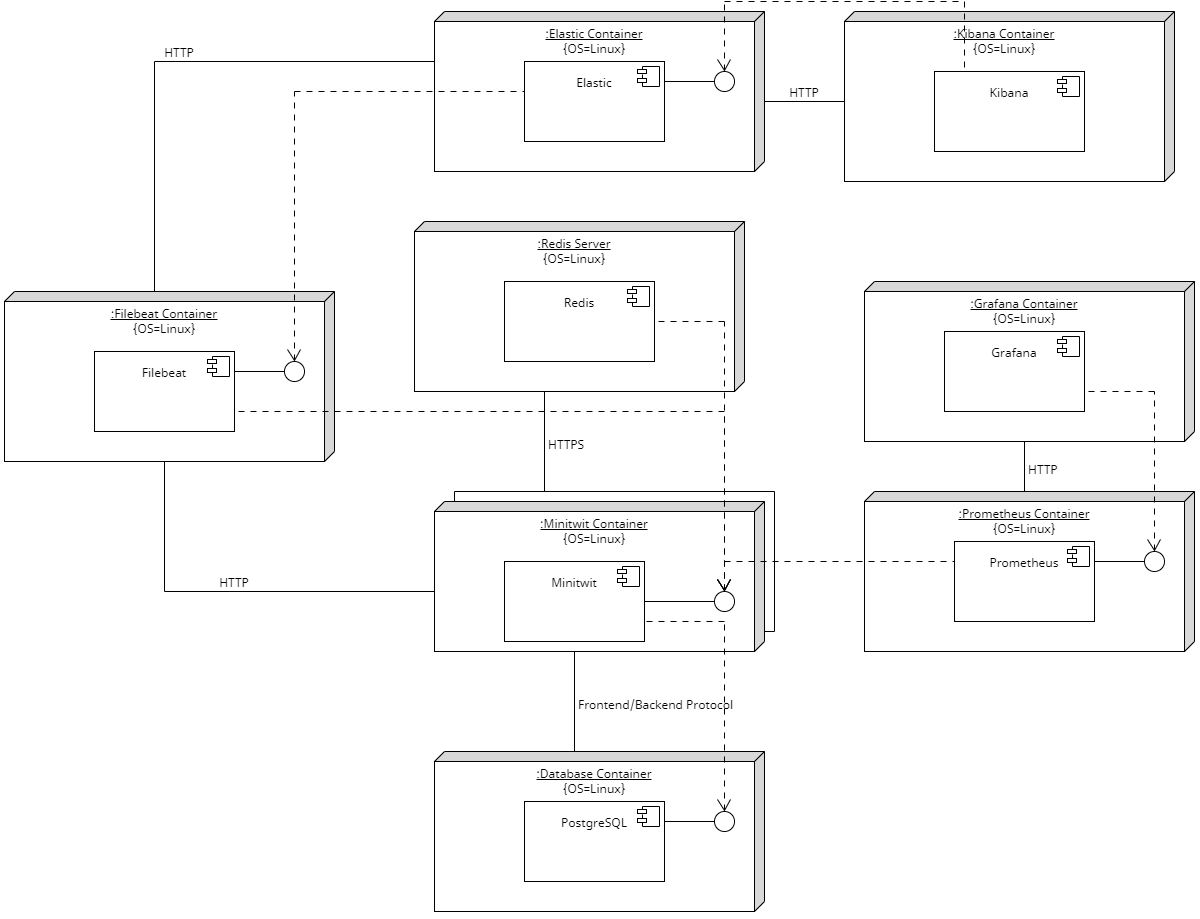
\includegraphics[width=0.9\textwidth]{images/Deployment_View_Picture.png}
\label{fig:deployment_view}
\caption{Minitwit deployment view}
\centering
\end{figure}

\subsection{Dependencies of the system (Mikkel)}
We list and briefly describe all technologies and tools we've applied and depend on:
\begin{itemize}
    \item Python and FastAPI for building the backend web-application.
    \item Jinja for displaying the frontend.
    \item PostgreSQL as database system.
    \item Docker for containerization.
    \item Vagrant for managing creation of virtual environments.
    \item DigitalOcean for hosting virtual environments on a remote server.
    \item GitHub Actions and Ansible for the CI/CD chain.
    \item SQLAlchemy as an ORM framework.
    \item Prometheus and Grafana for monitoring and visualising the state of the system.
    \item Postman for testing of the API.
    \item Elasticsearch, Filebeat and Kibana as a logging stack.
    \item Redis for storing state without hard consistency requirements (eg. total page views)
    \item Nginx and Heartbeat for a high-availablity setup with a staging and deployment server.
    \item Certbot for adding HTTPS to the website.
\end{itemize}
Arguments of our choices of technologies and tools used is provided in the respective sections of the report describing their usage in detail.

\subsection{Subsystem interactions}

Important interactions of subsystems

\subsection{State of the system (Mikkel)}
We have followed practices of software quality like testing, pair programming, code reviews and linting. To measure maintainability we have used Code Climate.

This allows accessing the state of the system whenever it is updated.

\subsection{Licences}
Finally, describe briefly, if the license that you have chosen for your project is actually compatible with the licenses of all your direct dependencies.

FOUND ON README.MD

\subsection{Weekly tasks (All) }


\subsubsection{Week 1 - Bug fixing the old program}
By importing the project to IntelliJ it auto-suggested to update the Python version from 2 to 3. We used shellcheck to lint the bash script.

\subsubsection{Week 2 - Refactoring the app in another language }

We listed possible frameworks, voted to exclude and then used a roulette to pick FastAPI. The process is described here \footnote{\url{https://docs.google.com/document/d/1EOrFKD0XFW5gxv1NycgtTuj9rO6dggau99LybLYIRq0/edit#heading=h.r8lyr8ciz36h }}. 

The arguments for FastAPI is how we could reuse the existing python code base and even reuse Jinja. Besides the ease of refactoring it was also familiar to some of us. 

We experienced some unexpected downsides.
\begin{itemize}

    \item The implementation of redirection for instance redirecting from a POST to another POST request would mean the loss of the original body and no way to pass it along. 
    \item Redirecting between different routes that return different status codes was also an unexpected challenge. 
    \item Since it is multi-threaded server it excludes the ability to have a global state and a session. We solved it with Starlette Session.
    \item The tests required to be translated to "pytest" framework in order to be utilised.
\end{itemize}

\subsubsection{Week 3 - Virtualisation and deployment to the server}

A new Docker feature called Dev Environments which gave us feature errors with mounting from files to containers and hot reloading .  

\subsubsection{Week 4 - Setting up CI/CD system }

Github Actions gave us a simple configuration process without needing additional hosted infrastructure. See section \ref{cicd}. 

\subsubsection{Week 5 - ORM }

Three ORMs have been considered and the arguments are mapped \footnote{\url{https://docs.google.com/document/d/1EOrFKD0XFW5gxv1NycgtTuj9rO6dggau99LybLYIRq0/edit#heading=h.auxry4rgtrx1}. A benchmarks repository was created \footnote{\url{https://github.com/MinitwitGroupI/ORM_Benchmarks }} and after a Github Discussion \footnote{\url{https://github.com/MinitwitGroupI/MiniTwit/discussions/57 }} a vote was held. The choice fell on the most popular choice for Python - SQLAlchemy - and it did not cause regret. 

\subsubsection{Week 6 - Monitoring }
Prometheus with Grafana is the most popular choice \footnote{https://stackshare.io/stackups/grafana-vs-nagios}. 

We checked our partner groups website and created issues for known issues \footnote{\url{https://github.com/organizationGB/DevOps/issues/23}} \footnote{\url{https://github.com/organizationGB/DevOps/issues/25}}. 



\subsubsection{Week 7 - Maintainability, external code analysing }

The Flake8 linter in our CI pipeline provides soft feedback that would not block builds but hint at potential problems. SonarQube and CodeClimate integrated perfectly with our repository but gave vastly different views on code quality than us. It required manually dismissing a lot of warnings about duplicated code which existed in our unit tests. It ended up being a burden rather than helpful.   


\subsubsection{Week 8 - EFK stack}

Significant issues were encountered when setting up EFK stack.
\begin{itemize}
    \item Poor support for creating custom user credentials.
    \item User credentials on Filebeat had to be manually hard coded.
    \item Deployment from localhost to production caused unexpected issues. Security features needed to be enabled for elastic search, filebeat and kibana. 
    \item EFK stack data flow was not set up properly in the example. Versions of EFK stack needed to be readjusted.
\end{itemize}

Postmortem exercises was completed. A bug was introduced an it was discovered with the help of logging.

\subsubsection{Week 9 - Security  assessment}
In order to asses the security of the program the team utilised "Metasploit", "OWASP ZAP" to detect any potential vulnerabilities inside the currently running application. This resulted in minor vulnerabilities related to HTML being discovered which were address in a later week.

In addition, the team debated on integrating "OWASP ZAP" in the CI/CD pipeline in order to asses if any future code would cause vulnerabilities. However, decided against it as it was not part of the assignment.

Lastly, we performed a security assessment on another group : 

\subsubsection{Week 10 - Scaling and rolling out updates }
We opted to go with the high-availability setup, since using a scalable deployment would require refactoring several components of our stack.
We already implemented deployments to a staging environment prior to production, so adding the staging server to our high-availability setup also provided us with rolling updates.  

\subsubsection{Week 12 - Encode your infrastructure setup }

Terraform did not provide additional benefits than our existing IaC with Vagrant. It worked for both provisioning and configuration management. Refactoring it into Terraform would require an almost 1:1 mapping of all functionalities along with extra configuration details (state).

\section{Process' perspective} \label{cicd}

\subsection{Team Organisation and Developer interaction (Ivar)} 

It was a goal to limit the number of tools.

Our team tried to employ as little various tools and methodologies as possible to streamline the organization of tasks and responsibilities. The only such tool was the Github issues functionality, which was particularly useful due to its integration with our codebase and its compatibility with a Kanban-style board visualization.

We strived to ensure that everyone worked on every aspect of the project, promoting a well-rounded understanding of each component. However, certain sections of the project were more esoteric and hacky, making it challenging for everyone to fully grasp the intricacies of every component. Despite this, our team's overall familiarity with each aspect of the project was satisfactory, and everyone contributed to most components.


\subsection{Stages and tools utilized in CI/CD chains (Ivar)}
Our team chose to use Github Actions as the primary CI/CD tool, as it is seamlessly integrated with our codebase on Github. This integration enables us to easily automate the process of building, testing and deploying our application with every commit on every pull request.

\subsubsection{Continuous Integration (CI)}
Upon each commit, Github Actions triggers a job that builds our application using Docker. This process creates a Docker image, which is then used as the environment for running our custom unit and integration tests.

For a pull request to be merged, it must successfully pass all unit and integration tests.

\subsubsection{Continuous Deployment (CD)}

Once a pull request has been merged with our main branch, our CD pipeline is automatically triggered. 
The first step in this pipeline is pushing the new versions our custom Docker images to our image repository. 

Then, using Ansible, we first deploy our entire application stack to a staging server. This environment allows us to verify the functionality and stability of our application before deploying it to production.

After successful deployment to the staging server, we run liveness tests using Postman. These tests are designed to validate the overall health and performance of our application, ensuring that it meets the necessary requirements for production deployment.

If our application successfully passes the liveness tests, it is then deployed to our production server.

\subsection{Organization of the repository}
\url{https://github.com/MinitwitGroupI/MiniTwit/blob/main/docs/CONTRIBUTE.md}
That is, either the structure of of mono-repository or organization of artifacts across repositories.
In essence, it has to be be clear what is stored where and why.

\textcolor{red}{this is already mostly explained in our CONTRIBUTE.md file}

\subsection{Branching strategy (Anders)}

We use the feature branches strategy for individual development. For releases \footnote{https://github.com/MinitwitGroupI/MiniTwit/releases} we achieved trunk based development by pushing into main and manually bundling a release. In order to push to main we had setup branch protection that require pull requests to be reviewed by at least one other team members\footnote{Initially two members were required to review it but we found it stifling to development and change it to one.}. Our branching philosophy is described here \footnote{https://github.com/MinitwitGroupI/MiniTwit/blob/main/docs/CONTRIBUTE.md}.

\subsection{Monitoring (Mads)}
We use Grafana and Prometheus to gather and visualize data on various aspects of our system, including endpoint hits, response times, total number of requests, CPU usage, and request duration distribution. These metrics are displayed across five different panels that provide a comprehensive overview of our system's performance. By monitoring these key metrics, we can quickly identify any issues that may arise and take action to ensure that our system is running smoothly and efficiently. You can find the dashboard here\footnote{\url{http://opsdev.gg:3000/d/DVJQxp-4k/minitwit-responses?orgId=1&from=now-24h&to=now}}.

todo: Explain why we find the metrics to be of interest.

\subsection{Logging (Anders)}

For logging we use the EFK stack. The Elasticsearch dashboard can be found on \url{http://opsdev.gg:5601} with the username helgeandmircea and password sesame0uvr3toi.

\subsection{Security Assessment}

In the security assessment we used "Metasploit" and "OWASP ZAP" in order to asses our security capabilities. However, all attacks failed to produce any significant results. 
In addition, another team  attempted to exploit the website but also did not produce any note worthy results. 
Lastly, the team asses the security capabilities of another team. This has results that resulted in the other teams database and cookies being compromised.
 

\subsection{Scaling and Load balancing (Anders)}

We have opted out of a scalable setup since this would require us to heavily refactor our infrastructure and separate our database from individual nodes. This would cost more with no added benefit in the confinement of the expected user growth before the deadline.  

\subsection{High-availability setup (Anders)}

We have opted for a high-available setup by using heartbeat using a guide provided by DigitalOcean \footnote{https://www.digitalocean.com/community/tutorials/how-to-create-a-high-availability-setup-with-heartbeat-and-reserved-ips-on-ubuntu-16-04}. This utilizes `floatip` which uses the DigitalOcean API to update the reserved IP to point at the other server when one is unavailable. 

????


\section{DevOps principles}

\subsection{What is DevOps}

Going by the DevOps Handbook \cite{devopshandbook} we have chosen a couple defining concepts to compare our result against. 

Todo: DevOps principles and how much we adhered to them (and how).

The categories are from here:
\url{https://github.com/itu-devops/lecture_notes/blob/master/sessions/session_05/README_TASKS.md}

\subsubsection{Flow}

Make work visible
Limit Work in Progress
Reduce Batch Sizes
Sometimes it was not possible to create small batch commits. The limitation being 

    Reduce the Number of Handoffs
    Continually Identify and Evaluate Constraints
    Eliminate Hardships and Waste in the Value Stream



\subsubsection{Feedback}

    See Problems as They Occur
    Swarm and Solve Problems to Build New Knowledge
    Keep Pushing Quality Closer to the Source
    Enable Optimizing for Downstream Work Centers


\subsubsection{Continual Learning and experimentation}

    Institutionalize the Improvement of Daily Work
    Transform Local Discoveries into Global Improvements
    Inject Resilience Patterns into Our Daily Work
    Leaders Reinforce a Learning Culture


\subsection{Another view - DevOps as a culture}

DevOps has enjoyed many different views through different eras \cite{devopsviewsthrougheras}. The supplemental book, The Phoenix Project \cite{thephoenixproject} and the guest lecture by Zander Havgaard from Eficode provides a fresh perspective of DevOps as a culture. 


Psychological safety: (Explain how we were at odds in the beginning when selecting a framework). 

"The Bus Factor" as repeated during the guest lecture which is the concept that no single developer should become key to development or infrastructure to the degree that progress can't occur without them. We failed in this regard. We each carved out our niche based on previous knowledge. While PR reviews occurred there was insufficient knowledge sharing for role shifting. 

\subsubsection{Ways we are not DevOps}

We don't follow the Toyota Kata. 

TDD... We could've written more code tests. Though with Postman we were able to test the availability of our infrastructure before deploying. Reflection: This seems like the typical case of tests being on the cutting block when time is scarce. 


\section{Lessons Learned Perspective}

\subsection{Issues and lessons learned (All)}


\subsubsection{Refactoring} 

Refactoring was a breeze because we choose FastAPI which allowed us to reuse big parts of the original Flask application. While Flask would've sufficed we managed to add better security through password encryption in our refactoring. 

\subsubsection{Evolution}

We were often blocked by upcoming tasks. We were waiting for the ORM task to finish so that we could create database migrations. We also anticipated the lecture about infrastructure as code since it would solve ????.

\subsubsection{Maintenance (Anders)}

Thanks to our monitor dashboards and Postman monitors we picked up on some infrequent outages. We could not verify whether some were caused by the simulator pausing or a problem on our end. We experienced at least three types of known outages:

\begin{enumerate}
    \item Outage during deployment while the Docker image was pulled and started. This was solved by our high-availability setup. 
    \item Didn't we experience some outages that were caused by the high-availability setup being misconfigured?
    \item The daily 5 AM outage. Through research we discovered that PostgreSQL by default restarts and does garbage collection and other maintanance. 
\end{enumerate}

Overall we felt that a minimal amount of maintenance is needed and would confidently hand over the project to another team. 

\subsection{Uptime}

The metrics in our SLA\footnote{https://github.com/MinitwitGroupI/MiniTwit/blob/main/docs/SLA.md} are based on postman and our monitoring dashboard. 





\subsection{Software Quality}



Static code analysis (the linting pipeline)

SonarQube through SonarCloud 

Code Climate

Terms we could use: SDLC, Technical debt


\subsection{Reflection (All)}

Also reflect and describe what was the "DevOps" style of your work. For example, what did you do differently to previous development projects and how did it work?

\subsection{Hand over}

We consider that no further maintenance is required. If a new group were to inherit our codebase we have created a document to guide them TODO. 

\section{Conclusion (All)}

Answer the question: Is what we've achieved DevOps?


\pagebreak
\printbibliography


\pagebreak
\section{Appendix}
\appendix


\section{Deployment View}
See next page
\label{appendix:DeploymentView}
\incgraph[documentpaper]
  [width=\paperwidth,height=\paperheight]{images/DeploymentView2.0.jpg}


\section{Hand over guide}
\label{appendix:handOverGuide}
Parts that need to be set up to inherit the codebase and deploy to a cloud server:
\begin{itemize}
    \item Local envionment variables: SSH\_KEY\_NAME, DIGITAL\_OCEAN\_TOKEN and AUTH\_KEY\_HEARTBEAT.
    \item GitHub Action Secrets: SSH\_HOST and STAGING\_SSH\_HOST.
\end{itemize}
To then deploy to a cloud server (in DigitalOcean), the "cloud\_deployment.md" guide in the GitHub repository should be followed.

In case the whole project is taken over, the following GitHub Actions Secrets would need to be set up:
\begin{itemize}
    \item DOCKER\_PASSWORD
    \item DOCKER\_USERNAME
    \item ELASTICSEARCH\_PASSWORD
    \item ENCRYPTION\_KEY
    \item PAT
    \item POSTGRES\_DB
    \item POSTGRES\_PASSWORD
    \item POSTGRES\_PORT
    \item POSTGRES\_SERVER
    \item POSTGRES\_USER
    \item POSTMAN\_API\_KEY
    \item REDIS\_HOST
    \item REDIS\_PASSWORD
    \item REDIS\_PORT
    \item SESSION\_SECRET\_KEY
    \item SSH\_HOST
    \item SSH\_KEY
    \item SSH\_USER
    \item STAGING\_SSH\_HOST
\end{itemize}

\section{Security Assessment (Partner Group)}
\label{appendix:securityAssessment}

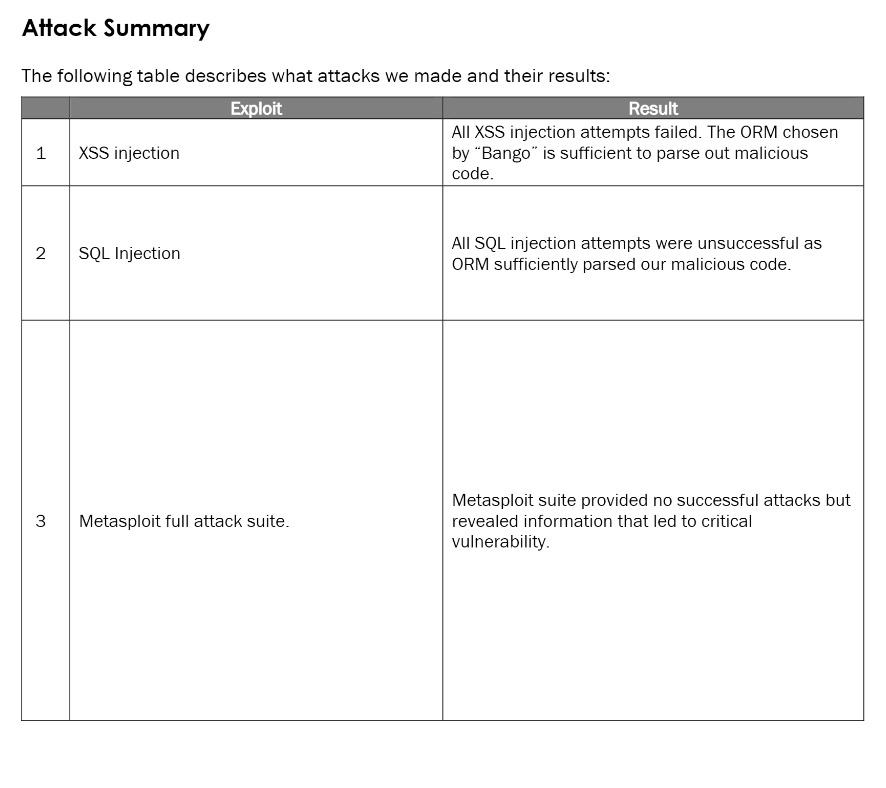
\includegraphics[width=1\textwidth]{images/Attack P1.png}

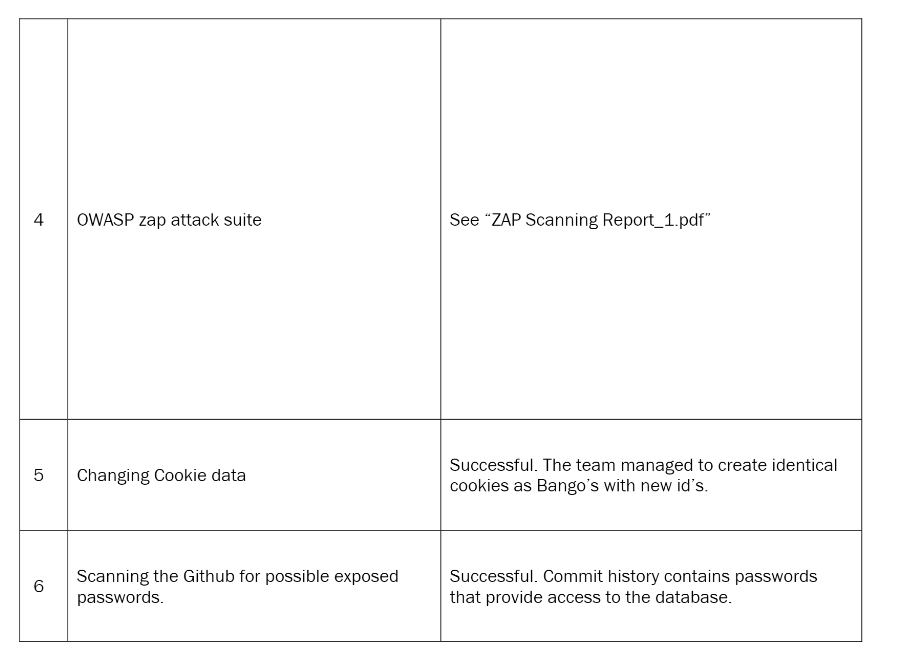
\includegraphics[width=1\textwidth]{images/Attack P2.png}
Read more :  \url{https://github.com/MinitwitGroupI/MiniTwit/blob/main/docs/security\%20report/Group\%20I\%20\%20-\%20Security\%20Assessment\%20Findings\%20Report.pdf}
\section{Current state of the application}
\label{appendix:currentState}
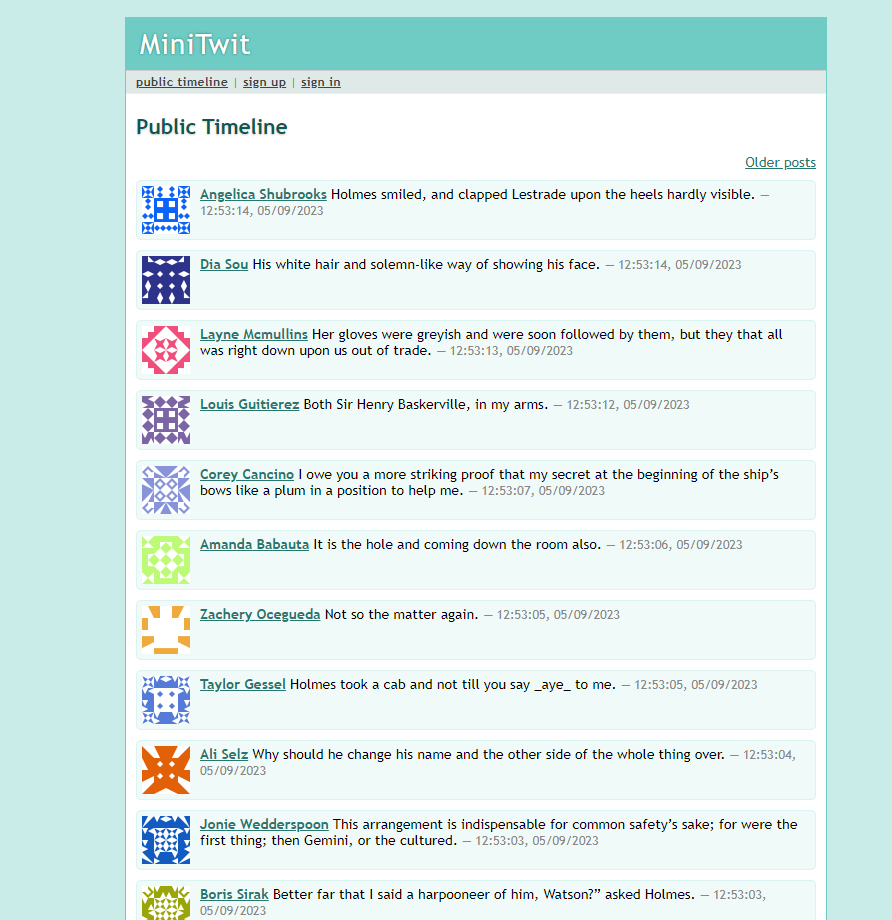
\includegraphics[width=1\textwidth]{images/OpsDev_screenshot.png}

\section{Monitoring Dashboard}
\label{appendix:monitoringDashboard}
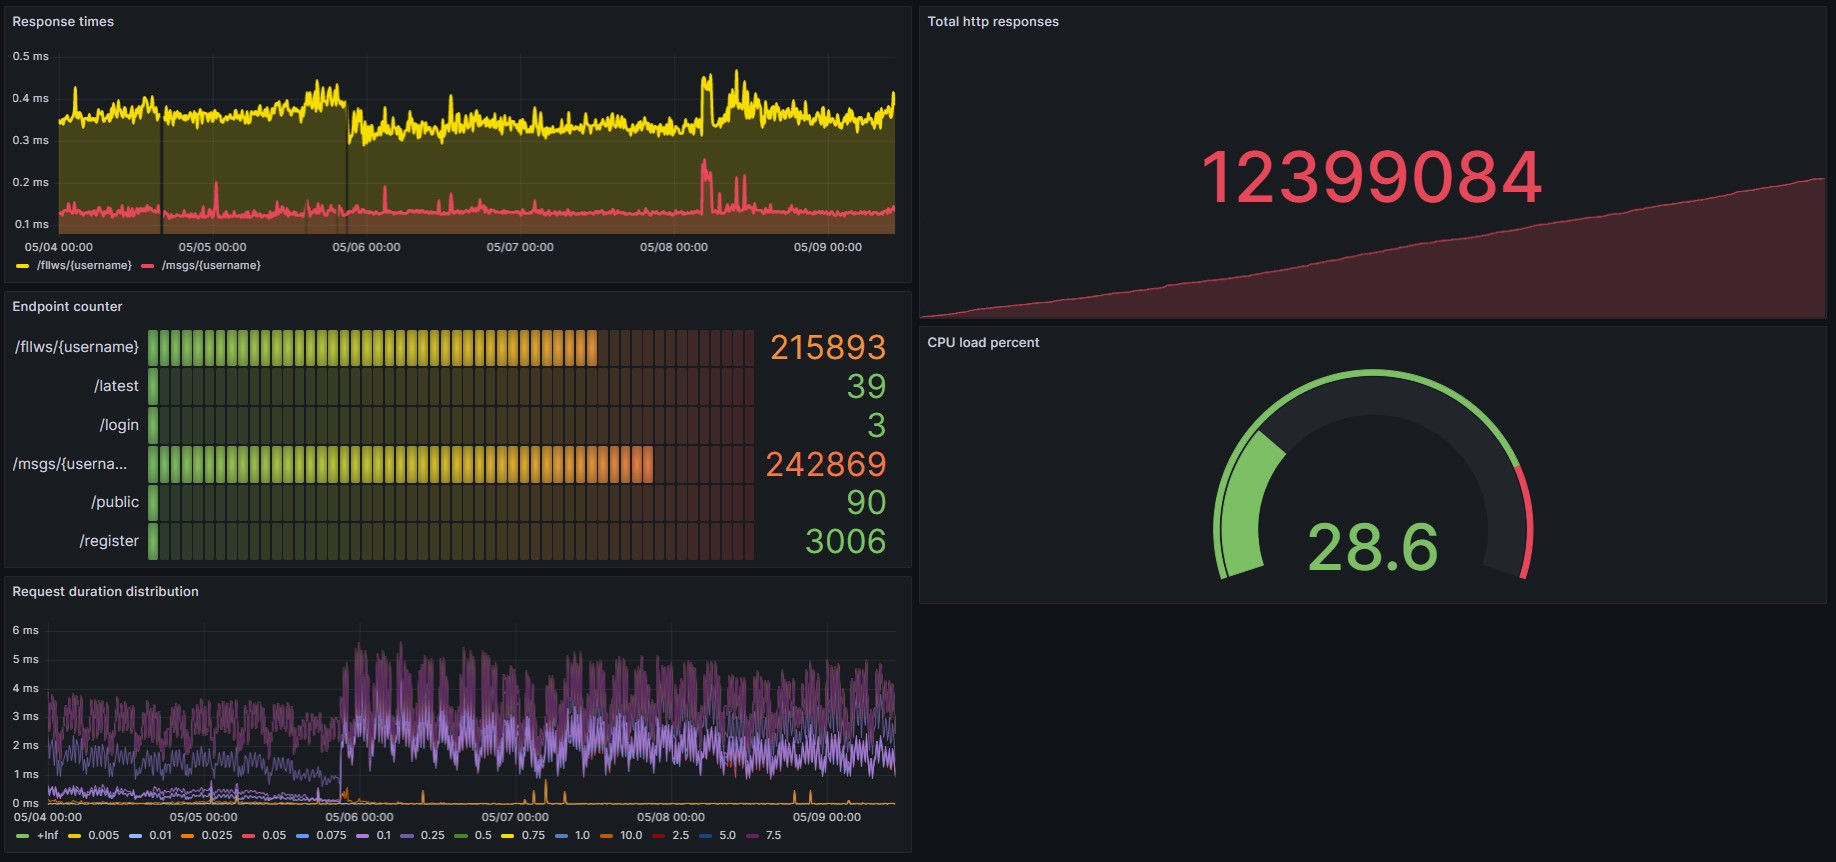
\includegraphics[width=1\textwidth]{images/MonitoringDashboard.jpg}

\section{Logging Dashboard}
\label{appendix:loggingDashboard}
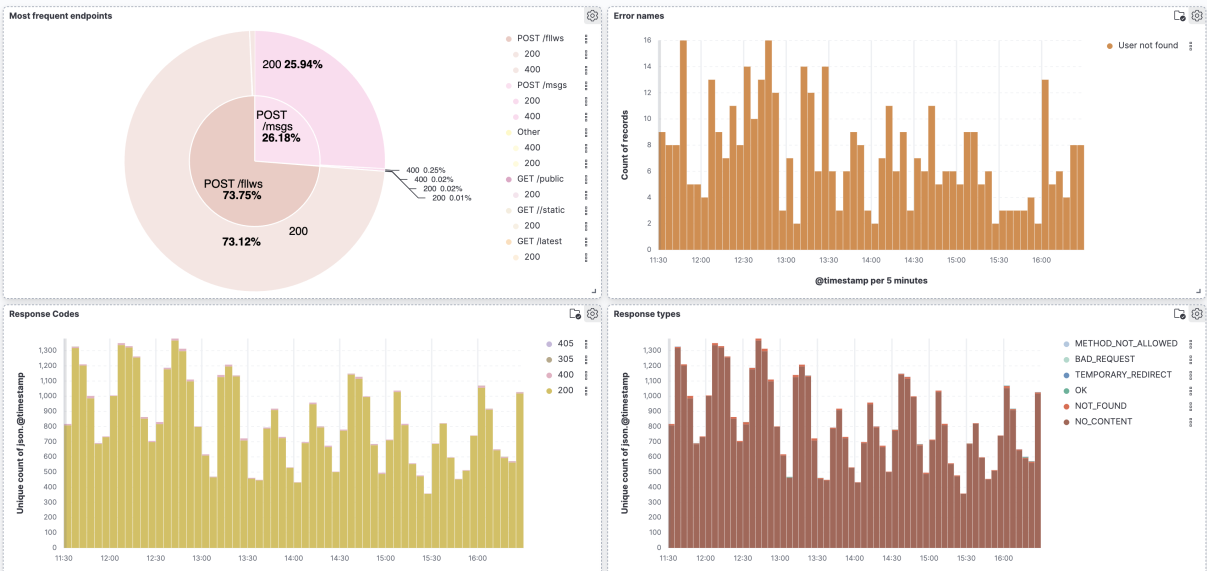
\includegraphics[width=1\textwidth]{images/LoggingDashboard.png}



\end{document}



